\section{Backup}
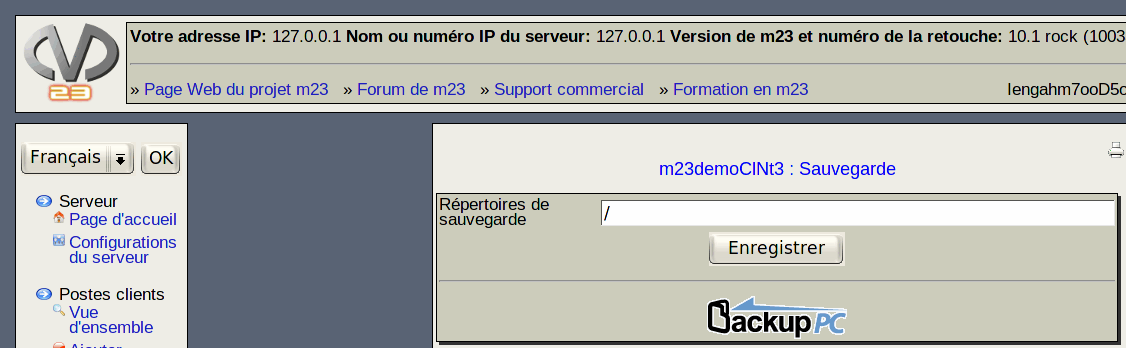
\includegraphics[scale=0.4]{/mdk/doc/manual/screenshots/de/client_backup.png} \\
In diesem Dialog k�nnen Sie alle Verzeichnisse des Clients angeben, von denen ein Backup erstellt werden soll. Geben Sie diese Verzeichnisse dazu durch Kommata getrennt in der Eingabezeile bei \textit{"Backup-Verzeichnisse"} an und klicken Sie anschlie�end auf \textit{"Speichern"}.\\
Das eigentliche Backup �bernimmt das Programm BackupPC, das Sie mit einem Klick auf das Icon starten k�nnen. In der BackupPC-Oberfl�che haben Sie Zugriff auf zus�tzliche Backup-Funktionen.\\
